
\section{Transferring models to Python}

\begin{figure}[h]
    \centering
    \addtolength{\leftskip} {-4cm}
    \addtolength{\rightskip}{-4cm}
    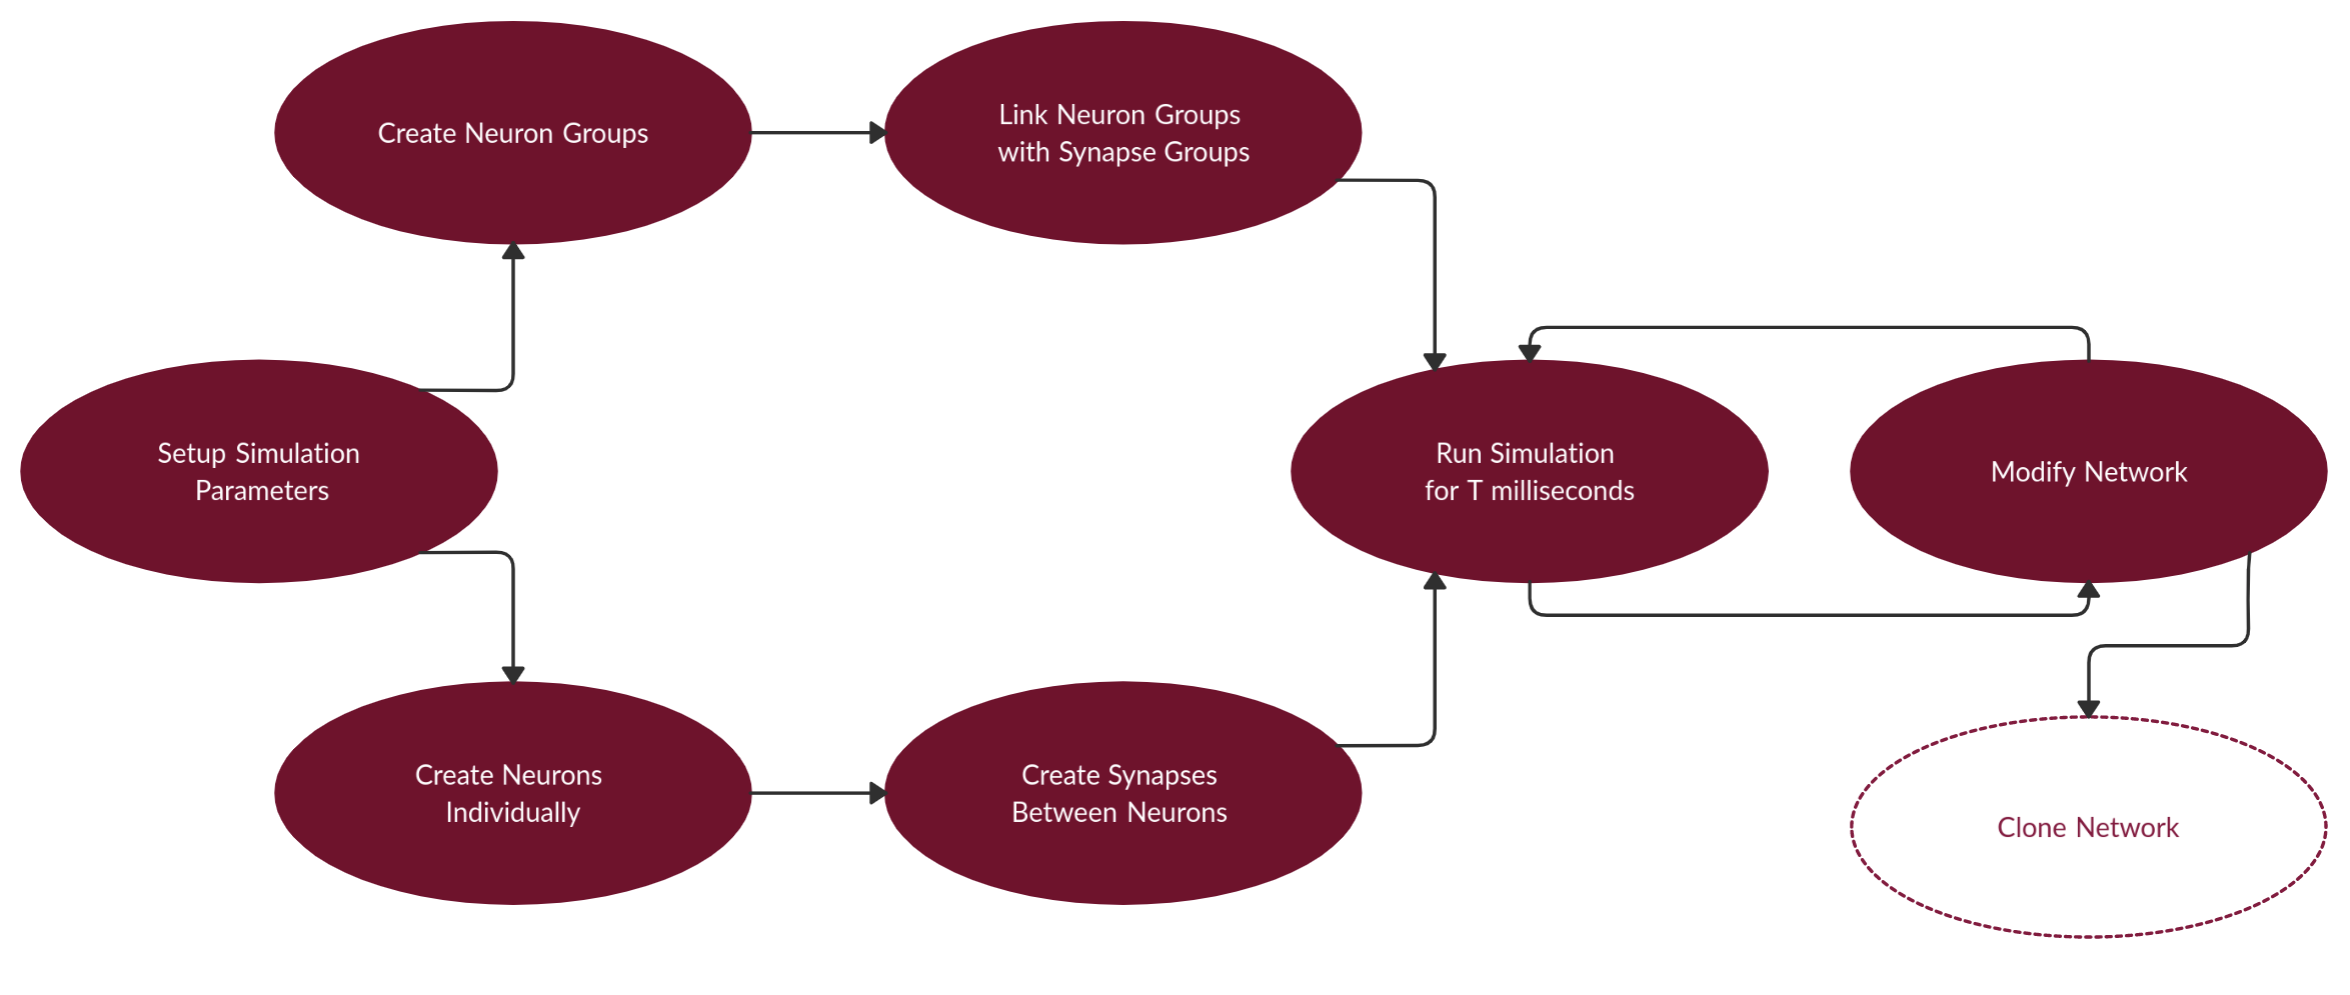
\includegraphics[width=1.3\linewidth]{figures/images/workflow.png}
    \caption[Workflow of the project simulation tooling]{A schematic that describes the intended workflow for preforming experiments with the simulation tooling that this chapter describes. Cloned simulations can be modified and continue to run in the same manner as their ancestor simulation.}
    \label{fig:workflow}
\end{figure}

In order to flexibly mix object oriented and functional programming paradigms,
I've chosen to develop these models in the Python programming language. Python has a healthy and active ecosystem of libraries and development practices
for scientific and statistical research to draw from. Of particular note are the
SciPy libraries, which provide a performant set of functions and objects that
speed up floating point arithmetic and vector mathematics. 

In figure \ref{fig:workflow}, the planned workflow for using the simulation is
mapped out, where the user can easily mix and match large probabilistically
generated networks and manually configured groups of neurons. It is in the
simulate and modify loop that experimentation can take place.

\subsection{Object oriented neurons}

In order to make the simulation as extendable as possible, I have chosen to
implement it in an object oriented manner, where functionality of the components
in the network is compartmentalised to the objects that should own said
functionality. For instance, each neuron owns its own state, state history, and
the functions that modify that state.

Another significant advantage of using object oriented programming in Python is
that objects can be deeply cloned using Python's \texttt{copy} library, a
significant benefit when it comes to duplicating networks for comparative
purposes.

\begin{figure}[h!]
    \centering
    % \addtolength{\leftskip} {-4cm} \addtolength{\rightskip}{-4cm}
    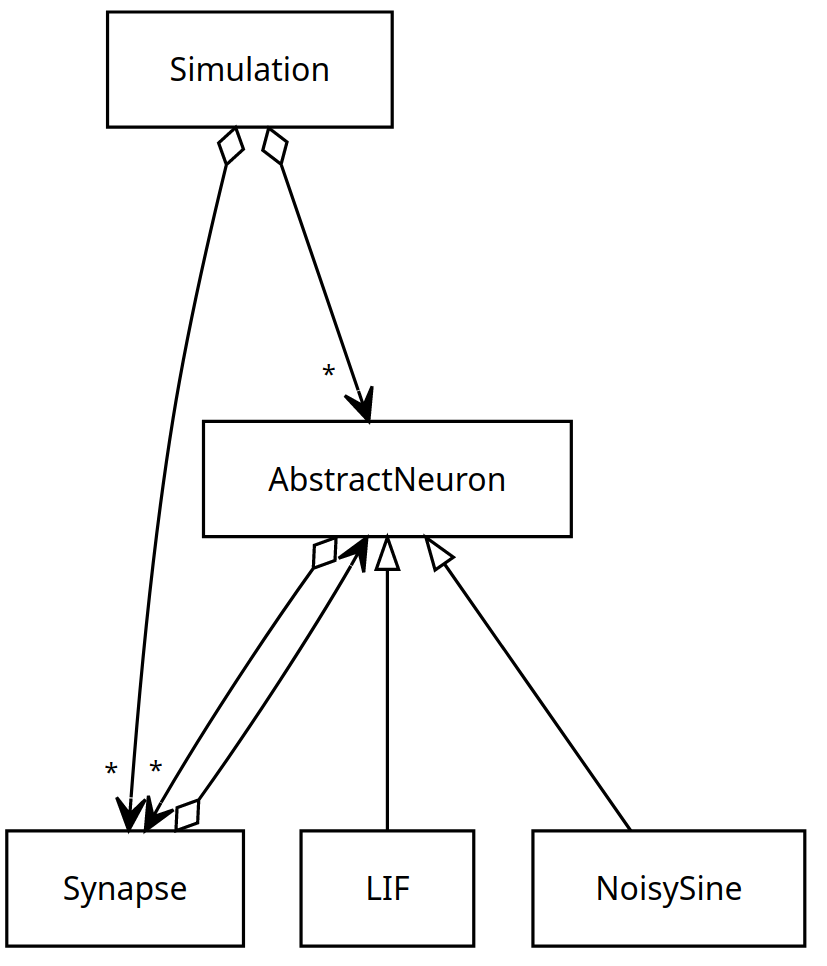
\includegraphics[width=0.5\linewidth]{figures/images/UML2.png}
    \caption[UML Diagram of objects in the simulation]{A UML Diagram of the
    objects in the simulation, where a Simulation class is composed of many
    AbstractNeurons and Synapses, and Neurons are implemented by multiple
    sub-classes.}
    \label{fig:uml}
\end{figure}

On a basic level, the hierarchy within the simulation is as follows: all neurons
and synapses belong to a \texttt{Simulation} object, and the neurons in the
network are doubly-linked with \texttt{Synapse} objects in-between. This is
illustrated in figure
\ref{fig:uml}, where neurons have been split into a base class \texttt{AbstractNeuron}
that holds the vector of input synapses and presents an interface to get the
neuron potential, but the specific implementation details are left to
\texttt{AbstractNeuron}'s implementations. One of these implementations is the
\texttt{LIF} neuron described earlier in this chapter, and the other is
the \texttt{NoisySine} neuron that uses overlapping sine-waves to generate an
output current. The core benefit of the these abstractions is
flexibility in the precise implementation of neurons. However, abstractions have
only been provided where necessary, as needless abstraction simply increases
system complexity and development time \autocite{shaw_abstraction_1984}.

The \texttt{Synapse} object holds the logic that pertains to STDP, and can
retrieve a list of the most recent spike times from the pre and post-synaptic
neurons in order to make STDP calculations. Once the weight delta from STDP is
calculated, the weight is modified and stored in the \texttt{Synapse}.

\FloatBarrier

\subsection{Network Topology}

In order to model the passing of information through the simulation, there were
several approaches that could be taken. In order to pick a solution, it is
necessary to map out the relationships between neurons in some sample topologies,
and the features that need to be supported by the synapses in such topologies. 

% TODO single file diagrams & quick explanation

\begin{figure}[h!]
    \begin{subfigure}{1\textwidth}
        \centering
        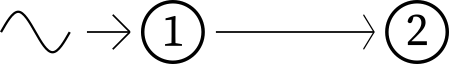
\includegraphics[width=0.35\linewidth]{figures/tops/top1.png}
        \caption{Neurons are connected in series, where each neuron has a single input}
        \label{fig:top1}
    \end{subfigure} \vspace{1ex} \\ 
    \begin{subfigure}{1\textwidth}
        \centering
        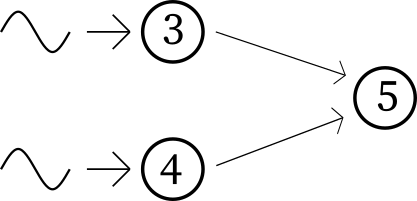
\includegraphics[width=0.35\linewidth]{figures/tops/top2.png}
        \caption{Neurons may have multiple synaptic inputs}
        \label{fig:top2}
    \end{subfigure} \vspace{1ex} \\
    \begin{subfigure}{1\textwidth}
        \centering
        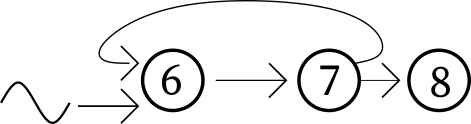
\includegraphics[width=0.35\linewidth]{figures/tops/top3.png}
        \caption{Multiple synapses may share a pre-synaptic neuron. "Recursive" feedback loops are found in the network.}
        \label{fig:top3}
    \end{subfigure}
    \caption[Sample network topologies for simulation]{Three sample network topologies for simulation. Numbered circles are spiking neurons, while waves mark an abstract input. Arrows between circles are synaptic connections.}
    \label{fig:tops}
\end{figure}

A simulation must be able to account for each of the sample topologies in figure
\ref{fig:tops} and the combinations thereof. The most complicated of these to
support is the "recursive loop" found in sub-figure \ref{fig:top3}, as without
placing restrictions on the network, the simulation could deadlock when two
neurons depend on the other's current potential. The two restrictions that can
be used are either to restrict the network such that recursive loops are
detected and prevented, or to provide guarantees that there is a significant
enough synaptic delay such that the deadlock can't occur. In order to do this, I
have implemented a runtime detection of recursive loops, so if a neuron that is
updating it's membrane potential for a time $T$ receives a request to update at
time $T$, it will throw an exception and end the simulation. 

\subsubsection{Stochastic generation of networks}

In order to create large networks with complex and varied parameters, it is
desirable to have functionality that can stochastically generate groups of
neurons. To support this, a wrapper class \texttt{NeuronGroup} has been written
that can create an arbitrary number of neurons, with each individual neuron
parameter drawn from a user provided distribution. Neuron groups can then be
probabilistically connected with synapses between their constituent neurons,
using the \texttt{SynapseGroup} helper class. These helper classes are not
involved in the actual running of the simulation, so advanced network set-ups
can still be manually created if an experiment requires.

\subsubsection{Using callable parameters}

To provide an extra layer of flexibility in network setup, both
\texttt{NeuronGroup} and \texttt{SynapseGroup} take Python \texttt{Callable}
objects as parameters, where the \texttt{Callable} is a function closure that
returns a sample from a distribution. As closures are functions that hold their
environment outside of their scope, this allows for lazily sampling from a distribution of the simulation user's choice on demand, for any
number of samples. Another advantage of this system is that the API surface of
the group wrapper classes is significantly reduced, which is beneficial as the
mental overhead of using large APIs has been shown to decrease programmer
performance \autocite{ellis_factory_2007,omar_active_2012}.